\documentclass[11pt,a4paper]{article}
\usepackage[utf8]{inputenc}
\usepackage[T1]{fontenc}
\usepackage[brazil]{babel}
\usepackage{lmodern}
\usepackage[margin=2.3cm]{geometry}
\usepackage{amsmath,amssymb,bm}
\usepackage{graphicx}
\usepackage{booktabs,longtable,array,tabularx,multirow}
\usepackage{xcolor}
\usepackage{listings}
\usepackage{caption}
\usepackage[hidelinks]{hyperref}
\usepackage{siunitx}
\sisetup{output-decimal-marker={,},group-separator={.},detect-all}

\graphicspath{{figs/}}
\newcolumntype{L}[1]{>{\raggedright\arraybackslash}p{#1}}
\lstset{language=C++,basicstyle=\ttfamily\scriptsize,columns=fullflexible,keepspaces=true,
  frame=single,framerule=0.3pt,rulecolor=\color{black!40},commentstyle=\color{black!55}\itshape,
  keywordstyle=\color{blue!50!black}\bfseries,breaklines=true,showstringspaces=false}
\newcommand{\code}[1]{\texttt{\detokenize{#1}}}
\newcommand{\sig}{\bm{\sigma}}
\newcommand{\eps}{\bm{\varepsilon}}
\newcommand{\D}{\mathbb{D}}

\title{Talude em Mohr--Coulomb no NeoPZ:\\
correções da plasticidade, fator de segurança e rebaixamento rápido do reservatório}
\author{Relatório técnico --- branch \code{branch_paper_mcc} de \code{diogocecilio/neopz-master}}
\date{8 de outubro de 2026}

\begin{document}
\maketitle

\begin{abstract}
Este relatório documenta o trabalho feito sobre o NeoPZ para analisar a estabilidade do talude do
projeto original \code{GeoMecDeterm} com o Mohr--Coulomb de projeção analítica em espaço de
Haigh--Westergaard rotacionado (Lira Cecílio, \emph{J.\ Eng.\ Math.}\ 157:10, 2026). Foram encontrados e
corrigidos erros no retorno ao Mohr--Coulomb, nas tangentes consistentes, na memória plástica, no
driver não linear e no pós-processamento; o código do artigo foi conferido com as equações (com três
erratas no texto). Dois projetos novos calculam o fator de segurança (FS) por aumento de gravidade e
por redução de resistência (SRM): \code{SlopeMohrCoulomb} (talude seco) e \code{SlopeDrawdown}
(solo saturado, rebaixamento rápido do reservatório, análise acoplada u--p de Biot e forças de
percolação, cenário de Ceron et al., 2025). Todos os resultados foram verificados: teste de Taylor da
tangente, convergência quadrática de Newton, convergência do FS com o refinamento, equilíbrio-limite
de Bishop com o mesmo campo de poropressão e uma solução independente da percolação permanente.
\end{abstract}

\tableofcontents

%=====================================================================================================
\section{Escopo e histórico}

Pedidos atendidos, na ordem em que foram feitos:
\begin{enumerate}
\item criar um projeto que simule o talude (\code{SlopeAnalysis.cpp/.h}, \code{main.cpp} de
  \code{Projects2/GeoMecDeterm}) com o Mohr--Coulomb melhorado; procurar inconsistências e erros
  (retorno ao critério, matriz tangente consistente, memória plástica, todo o código) e corrigi-los,
  reaproveitando o código existente onde não houvesse erro; limpar e documentar; resolver por
  aumento de carga (gravidade) e por redução de resistência;
\item verificar inconsistências entre o artigo e o código;
\item manter o pós-processamento original (\code{PostPlasticity}, \code{CreatePostProcessingMesh},
  \code{PostProcessVariables});
\item ajudar com as funções \code{CreatePressureMesh} e \code{CreateCompMesh} de um problema
  poroplástico (u--p) para o talude;
\item em um projeto novo, sem alterar o atual, simular o talude saturado com o nível d'água no
  topo e o rebaixamento rápido do reservatório, como em Ceron et al.\ \cite{ceron2025}, calculando o
  FS pelo mesmo procedimento de estabilidade;
\item este relatório.
\end{enumerate}

\begin{table}[h]
\centering\small
\begin{tabular}{@{}lL{11.5cm}@{}}
\toprule
commit & conteúdo \\
\midrule
\code{bb77c0a} & biblioteca: retornos ao Mohr--Coulomb, tangentes consistentes, memória plástica, driver não linear \\
\code{22a9615} & projeto \code{SlopeMohrCoulomb} (FS por aumento de gravidade e SRM, refinamento da zona plástica) \\
\code{cb6fd46} & pós-processamento original mantido; variáveis \code{POrder}, \code{Coesion}, \code{Atrito} no material \\
\code{be1d4ef} & projeto \code{SlopeDrawdown}; instanciação u--p do Mohr--Coulomb; \code{SlopeModel.h} \\
\bottomrule
\end{tabular}
\caption{Commits sobre o \code{e3eb3a4} (upstream).}
\end{table}

%=====================================================================================================
\section{Convenções e modelo constitutivo}

\paragraph{Voigt.} Tensores em \code{TPZTensor} na ordem $(xx,xy,xz,yy,yz,zz)$; deformações com
cisalhamento de engenharia ($\gamma_{xy}=2\varepsilon_{xy}$) e tensões com componentes tensoriais,
de modo que $\sig = \D^e\eps$ com $\D^e_{xy,xy}=G$ (convenção do artigo, Eq.~22 e 26, e de
\code{TPZElasticResponse::De}). Todas as tangentes são $\partial\sig/\partial\eps$ nessa convenção e
entram diretamente em $\int B^T\D B$. Tração positiva; na análise u--p a poropressão $p$ é positiva em
compressão e $\sig_{\text{total}}=\sig'-\alpha p\,\mathbf I$.

\paragraph{Critério e retorno.} Em tensões principais $\sigma_1\ge\sigma_2\ge\sigma_3$,
\begin{equation}
f(\sig) = (\sigma_1-\sigma_3) + (\sigma_1+\sigma_3)\sin\phi - 2c\cos\phi \le 0 .
\end{equation}
O modelo do artigo (\code{TPZPlasticStepVoigt<TPZYCMohrCoulombPV2>}) projeta o preditor elástico em
forma fechada no espaço de Haigh--Westergaard rotacionado, com quatro regiões (plano principal,
duas arestas, ápice), e devolve a tangente consistente espectral
\begin{equation}
\D^{ep} = \sum_{i,j}\frac{\partial\sigma_i}{\partial\varepsilon^{tr}_j}\,\mathbf E_i\otimes\mathbf E_j
 + \sum_{i\ne j}\frac{\sigma_i-\sigma_j}{\varepsilon^{tr}_i-\varepsilon^{tr}_j}\,\mathbb E_{ij},
\end{equation}
termo coaxial mais correção de rotação dos autovetores (Eq.~28--37 e Listing~1 do artigo). O modelo
antigo \code{TPZPlasticStepPV<TPZYCMohrCoulombPV>} (Souza Neto, Box 8.5, iterativo) foi corrigido e
mantido para verificação cruzada.

\paragraph{Redução de resistência e aumento de gravidade.} No SRM, $c_F=c/F$, $\phi_F=\arctan(\tan\phi/F)$
e $\psi=\phi$ (associativo). No aumento de gravidade todas as forças de volume são multiplicadas por
$\lambda$; para Mohr--Coulomb isso equivale a dividir só $c$ por $\lambda$, de modo que
$\text{FS}_{\text{grav}}\ge\text{FS}_{\text{SRM}}$ quando $\phi>0$.

%=====================================================================================================
\section{Erros corrigidos na biblioteca}\label{sec:bugs}

A Tabela~\ref{tab:bugs} lista as correções (commit \code{bb77c0a}, e as duas linhas finais dos
commits \code{cb6fd46} e \code{be1d4ef}). Antes do commit, quatro revisões adversariais encontraram
regressões que as primeiras versões das correções introduziam, todas evitadas:
vetor \code{fmatprop} nulo de placeholder tratado como propriedade do ponto (zeraria $c$); caminho
antigo de \code{ApplyStrainComputeDep} necessário ao Cam-Clay/Drucker--Prager (restaurado; só o
Mohr--Coulomb usa o novo); leitura de $\psi$ de \code{fmatprop[2]} (revertido para $\psi=\phi$);
\code{Phi()} do Voigt abortando para Von Mises/Tresca (funções de escoamento implementadas); e a
restauração de $\eps^*/\sig^*$ em \code{TPZElasticResponse}, que regrediria a elasticidade porosa
(revertida e documentada como pendência).

{\small
\begin{longtable}{@{}L{3.1cm}L{4.6cm}L{3.4cm}L{4.4cm}@{}}
\caption{Problemas encontrados e correções.}\label{tab:bugs}\\
\toprule
Arquivo & Problema & Efeito & Correção\\
\midrule\endfirsthead
\toprule
Arquivo & Problema & Efeito & Correção\\
\midrule\endhead
\code{TPZPlasticStepPV.cpp} & autovetores de $\eps^{tr}$ com $\gamma$ no slot $xy$; tangente derivada em relação a $\eps$ tensorial & tangente errada até no regime elástico (Taylor ordem 1, $D_{xy,xy}=2G$); Newton linear & autossistema único de $\sig^{tr}$ ($\varepsilon_i-\varepsilon_j=(\sigma_i-\sigma_j)/2G$); colunas de cisalhamento $\times\tfrac12$\\
\code{TPZPlasticStepPV.cpp} & termo de rotação com os autovalores de teste (Souza Neto C.14 usa os projetados) & rigidez de rotação elástica nos pontos plásticos & autovalores projetados\\
\code{TPZPlasticStepPV.cpp} & \code{tempMat} acumulado entre pares $(i,j)$; \code{Tangent +=} sem zerar & tangente 3D errada; lixo em \code{Dep} & matriz por par; \code{Redim(6,6)}\\
\code{TPZPlasticStepPV.h/.cpp} & \code{fReductionFactor()} $=0$; SRM só com \code{fmatprop[0]>1e-3} & $c/0$; redução ignorada sem propriedades por ponto & padrão 1; \code{LocalCriterion()} com propriedades do ponto e redução, sem composição\\
\code{TPZPlasticStepPV.cpp} & \code{ApplyStrainComputeDep} chamava \code{ProjectSigmaDep} (\code{DebugStop} no MC); \code{Phi()} sem parâmetros locais & teste de tangente inutilizável; \code{Yield} sem redução & especialização MC via \code{ApplyStrainComputeSigma}; \code{Phi} com \code{LocalCriterion()}\\
\code{TPZYCMohrCoulombPV.h/.cpp} & \code{GetLocalMatState} com \code{DebugStop}; \code{ChangeLocalMatParameters} recomputava de \code{fmatprop} & SRM ignorado & redução dos parâmetros correntes numa cópia; $\psi=\phi$\\
\code{TPZYCMohrCoulombPV.cpp} & validade das arestas com tolerância absoluta $10^{-12}$ & retorno de aresta enviado ao ápice & tolerância relativa\\
\code{TPZYCMohrCoulombPV.cpp} & $\psi=0$ no ápice ($0/0$); \code{k_proj} indefinido no ramo elástico; \code{SigmaElastPV} & NaN; endurecimento zerado & guardas; \code{k_proj = k_prev}; índices\\
\code{TPZYCMohrCoulombPV2.cpp} & ramo elástico \code{alphan = alphan1} (sobrescreve a entrada) & memória com lixo & \code{alphan1 = alphan}\\
\code{TPZYCMohrCoulombPV2.cpp} & ápice com Jacobiano $-10^{-11}$; teste elástico $\Phi<0$; \code{m_type = 1} em todas as regiões & tangente espúria; regiões indistinguíveis & Jacobiano nulo; $\Phi\le0$ (Eq.~56); tipos 1, 2, 3, $-1$\\
\code{TPZYCMohrCoulombPV2.h/.cpp} & \code{YieldFunction}, \code{SetLocalMatState}, \code{ChangeLocalMatParameters}, \code{Print} vazios; funções sem \code{return}; $\psi$ ignorado & SRM impossível; UB & implementados (Eq.~44, 45, 49); \code{DebugStop} se $\psi\ne\phi$\\
\code{TPZPlasticStepVoigt.cpp/.h} & \code{hvarnew} não inicializado; ER não repassado ao critério & UB; projeção com módulos diferentes (ordem 1) & inicializado; ER repassado\\
\code{TPZPlasticStepVoigt.cpp/.h} & sem fator de redução; cópia descartava \code{fN}; \code{ClassId()=0}, \code{Read/Write} vazios; \code{Phi()=0}; \code{ApplyStrainComputeDep} nulo & SRM impossível; serialização inútil & \code{SetStrengthReductionFactor}, \code{LocalCriterion()}, cópia, serialização, \code{Phi}\\
\code{TPZPlasticStepVoigt.cpp} & ramo elástico reconstruído pela decomposição espectral & erro $\sim10^{-8}$ com autovalores repetidos & $\sig=\sig^{tr}$; no plástico só a correção\\
\code{TPZYCTrescaVoigt}, \code{TPZYCVonMisesVoigt} & mesmo \code{alphan = alphan1}; \code{YieldFunction}$=$\code{DebugStop} & endurecimento corrompido & corrigidos\\
\code{TPZElasticResponse.cpp} & \code{operator=} não copiava $\sig^*$ & cópia incompleta & corrigido\\
\code{TPZPlasticState.h} & cópia: \code{fmatpropinit(source.fmatprop)} & reduções compostas & \code{fmatpropinit(source.fmatpropinit)}\\
\code{TPZMatElastoPlastic_impl.h} & \code{m_m_type} não gravado; \code{m_u} só com o último incremento & \code{FailureType} sempre 0; deslocamento errado & gravados; \code{m_u += du}\\
\code{TPZMatElastoPlastic_impl.h} & ER não linear gravado fora do commit & escrita fora de \code{fUpdateMem} & ER local\\
\code{TPZMatElastoPlastic_impl.h} & invariantes de deformação com $\gamma$ no slot tensorial & $J_2(\eps^p)$ errado & conversão $\gamma\to\varepsilon$\\
\code{TPZMatElastoPlastic_impl.h/.h} & cópia sem \code{m_force0}/\code{fExactSolution}; ponteiro não inicializado; \code{EEXACT}; \code{NSolutionVariables} & UB; pós-processamento errado & corrigidos\\
\code{TPZMatElastoPlastic2D_impl.h} & \code{auto bc_with_memory} (cópia de toda a memória por ponto); BC tipo 4 em \code{Val2} compartilhado & custo $O(n^2)$; corrida entre threads & referência; tração local\\
\code{TPZMatWithMem.h} & \code{operator=} sem \code{return} & UB & corrigido\\
\code{pzelastoplasticanalysis.cpp} & buscas lineares clonavam a malha inteira a cada iteração; a dicotômica não testava o passo completo & vazamento; convergência linear & avaliação in loco; passo completo aceito se reduzir $\|R\|$\\
\code{pzelastoplasticanalysis.cpp} & \code{ELineSearch::None} com \code{fSolution} vazio; sem saída para NaN; aceitava passo não convergido; ponteiros nulos em \code{SetAllCreateFunctionsWithMem} & falhas; memória corrompida & corrigidos\\
\code{pznonlinanalysis.cpp} & \code{sol += prevsol} em cópia descartada & Newton sem busca linear não converge & \code{fSolution += prevsol}\\
\code{TPZMatElastoPlastic_impl.h/.h}, \code{TPZYCMohrCoulombPV2.h} & \code{POrder}, \code{Coesion}, \code{Atrito} do pós-processamento original inexistentes & variável desconhecida & $c$ e $\phi$ do critério local (já reduzidos)\\
\code{TPZMatPoroElastoPlasticUP.cpp}, \code{TPZPlasticStepVoigt.h} & material u--p instanciado só para Cam-Clay; falta \code{LastProjectionFailed()} & Mohr--Coulomb indisponível no u--p & instanciação explícita; projeção fechada nunca falha\\
\bottomrule
\end{longtable}}

\paragraph{Pendências documentadas (não alteradas).} \code{TPZPlasticStepPV::ApplyStressComputeStrain}
e \code{ApplyLoad} (não usados) continuam incorretos; o caminho Cam-Clay/Drucker--Prager/Sandler de
\code{TPZPlasticStepPV} usa a tangente antiga (\code{ProjectSigmaDep}), fora da convenção de cisalhamento
de engenharia; \code{TPZElasticResponse::ComputeStress/ComputeStrain} ignoram $\eps^*/\sig^*$ desde o
commit \code{e16d8bc} (restaurar exige corrigir \code{TPZPorousElasticResponse::ComputeStress}).

%=====================================================================================================
\section{Artigo $\times$ código}

O código foi conferido com uma transcrição literal das equações em numpy, com uma referência
independente (Souza Neto, Box~8.5) e com a projeção exata de ponto mais próximo por conjunto ativo,
em \num{24000} estados aleatórios: tabelas 4--6, Eq.~57--58 e o código coincidem (tensão $10^{-14}$,
Jacobiano $4\cdot10^{-16}$); seleção de região (Eq.~59--61) idêntica; tangente (Eq.~29--37 e Listing~1)
igual ao código e às diferenças finitas ($1{,}7\cdot10^{-8}$). Divergências do código em relação ao
artigo, corrigidas no código: Jacobiano do ápice ($-10^{-11}$, artigo: $\D=0$), teste elástico
$\Phi_1<0$ (artigo: $\Phi_1\le0$) e $\psi$ ignorado sem aviso. Erratas do texto (sem efeito no código):
\begin{itemize}
\item a Eq.~(54) está multiplicada por 432 (falta o fator $1/432$); o minimizador não muda;
\item as tabelas 4--6 trazem ``$\sin\phi^2$'' onde deve ser $\sin^2\phi$;
\item a Eq.~(28) deveria usar $(\mathbf v^{\varepsilon}_{jj})^T$ (mapa de deformação) e é só a parte
  coaxial; a Eq.~(29) implementada ($\mathbf A+\mathbf R_V$) está correta.
\end{itemize}
No exemplo da sapata do artigo (\code{Projects2/PlasticityTestsMohrCoulomb}, removido do branch) o
driver aplicava pressão (Neumann) e não o recalque prescrito da Seção~5.1, não calculava $P=R/B$, usava
a regra de 6 pontos do P2 (o artigo usa 3), \code{fBigNumber} $\approx6{,}7\cdot10^{16}$ e tolerâncias
absolutas de $10^{-6}$, e aceitava incrementos não convergidos.

%=====================================================================================================
\section{Projeto \code{SlopeMohrCoulomb}: talude seco}\label{sec:slope}

\begin{figure}[t]
\centering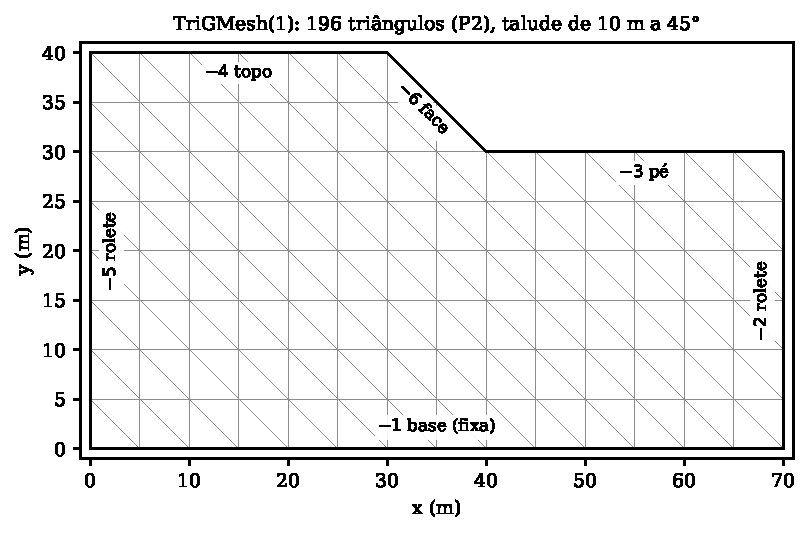
\includegraphics[width=0.78\textwidth]{fig_mesh.pdf}
\caption{Geometria e malha inicial (\code{TriGMesh(1)} de \code{SlopeModel.h}): domínio
$70\times40$~m, talude de 10~m a $45^\circ$, ids de contorno.}\label{fig:mesh}
\end{figure}

\paragraph{Dados.} $E=\SI{20000}{kPa}$, $\nu=0{,}49$, $c=\SI{10}{kPa}$, $\phi=\psi=30^\circ$,
$\gamma=\SI{20}{kN/m^3}$; triângulos P2; base fixa e laterais em rolete (Figura~\ref{fig:mesh}).

\paragraph{Algoritmo (\code{SlopeAnalysis.h}).}
\begin{itemize}
\item \code{Reset()}: memória plástica virgem e análise nova (\code{TPZSkylineStructMatrix} com threads,
  $LDL^T$; as tangentes são simétricas).
\item \code{Newton()}: Newton--Raphson com a tangente consistente, retrocesso em $\|R\|$ guardando o
  melhor iterado, saída por divergência; $\|R\|\le10^{-8}\|F_{ext}\|$.
\item \code{Continuation()}: a partir de um estado de equilíbrio aumenta o parâmetro; se Newton converge
  aceita o estado (memória plástica) e aumenta o passo ($\times1{,}5$); se falha descarta a tentativa e
  divide o passo por 2; para quando o passo $<0{,}2\%$ do parâmetro. O FS é o último valor convergido.
\item \code{GravityIncrease()}: parâmetro $\lambda$ multiplicando a força de volume.
  \code{StrengthReduction()}: gravidade total aplicada por continuação com $F_0=1$ (dividido por 2 até
  haver equilíbrio, o que permite FS $<1$) e depois continuação em $F$.
\item \code{MarkPlasticZone()}/\code{Refine()}: marca os elementos com $\sqrt{J_2(\eps^p)}\ge10\%$ do
  máximo no colapso do GI e do SRM, divide-os com balanceamento 2:1 e renumera a banda.
\item \code{PostPlasticity()}, \code{CreatePostProcessingMesh()}, \code{PostProcessVariables()}: as do
  projeto original, com \code{POrder}, \code{Atrito}, \code{Coesion} (valores efetivos no ponto, já
  reduzidos), \code{StrainPlasticJ2}, \code{FailureType} e o deslocamento total.
\end{itemize}

\paragraph{Driver original --- por que foi reescrito.} O SRM era inalcançável (\code{LoadingRamp} e
\code{ApplyGravityLoad} eram \code{DebugStop}; sem \code{fmatprop} a redução era ignorada pela biblioteca;
\code{ShearRed} gravava $c_0/\text{FS}$ e a biblioteca dividia de novo); as tentativas da bissecção não
eram independentes; critérios absolutos de convergência; \code{FS}/\code{FSOLD} não inicializados
(divisão por zero); arc-length aceitava passos não convergidos; construtor de cópia raso com destrutor
que apagava as malhas; skyline simétrica com a tangente não simétrica do caminho antigo; sem
renumeração de banda após o refinamento.

%=====================================================================================================
\section{Verificação do talude seco}\label{sec:verif}

\paragraph{Teste de Taylor no ponto material.} Para estados $\eps$ em referencial girado aleatoriamente,
incluindo autovalores repetidos, o resto
$E(\alpha)=\|\sig(\eps+\alpha\Delta\eps)-\sig(\eps)-\alpha\D\Delta\eps\|$ deve cair com ordem 2
(Eq.~63--65 do artigo). A Figura~\ref{fig:taylor} confirma ordem 2 no plano principal e nas duas arestas
para os dois modelos e resto nulo (exato) no regime elástico e no ápice (\code{check}). Antes das
correções o modelo antigo tinha ordem 1 em todos os regimes, inclusive no elástico. As tangentes são
simétricas ($|\D-\D^T|/|\D|<2\cdot10^{-14}$), o que legitima a fatoração $LDL^T$.

\begin{figure}[t]
\centering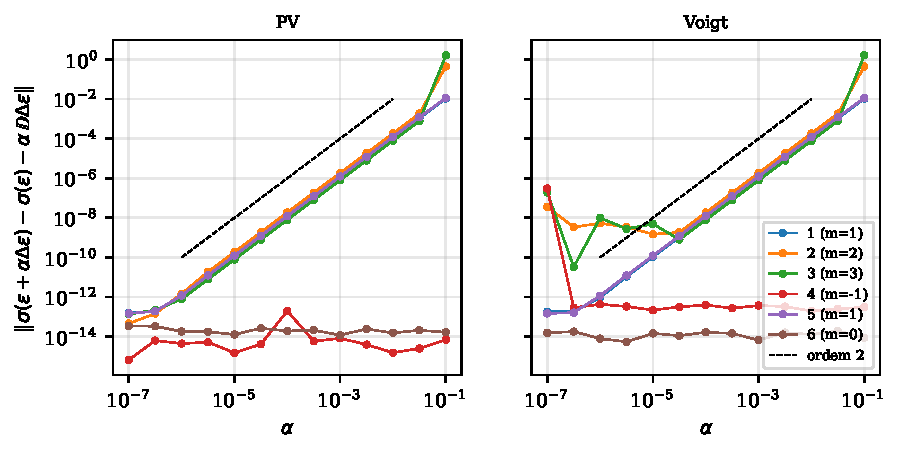
\includegraphics[width=0.92\textwidth]{fig_taylor.pdf}
\caption{Teste de Taylor da tangente consistente (\code{SlopeMohrCoulomb check}): resto de segunda
ordem em escala log-log; $m$ = região de retorno (1 plano principal, 2 e 3 arestas).}\label{fig:taylor}
\end{figure}

\paragraph{Newton.} Com a tangente consistente a convergência global é quadrática
(Figura~\ref{fig:newton}), p.ex.\ $\|R\|/\|F\|$: $4\cdot10^{-5}\to4\cdot10^{-8}\to10^{-13}$.

\begin{figure}[t]
\centering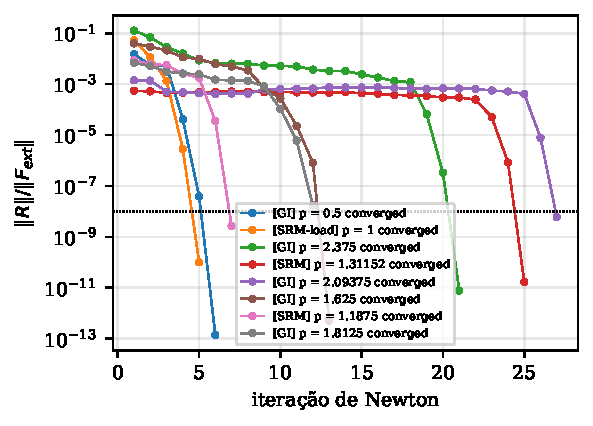
\includegraphics[width=0.55\textwidth]{fig_newton.pdf}
\caption{Histórico de Newton em passos convergidos das continuações (talude seco, \code{SLOPE_VERBOSE=1}).}\label{fig:newton}
\end{figure}

\paragraph{FS e refinamento.} A Tabela~\ref{tab:fsdry} e a Figura~\ref{fig:fsdry} mostram o FS em cada
ciclo de refinamento. Os dois modelos constitutivos, independentes, dão o mesmo FS dentro da
tolerância da continuação, e ambos convergem para o equilíbrio-limite (Bishop simplificado, busca de
círculos em script independente: 1,857 por gravidade e 1,209 por SRM). A malha grossa superestima o FS
por gravidade (mecanismo raso junto à face, Figura~\ref{fig:mechdry}). Com $\nu=0{,}3$ (ciclo 5) o FS é
1,789 e 1,207: sem travamento volumétrico relevante.

\begin{table}[h]
\centering\small
\begin{tabular}{@{}rrcccc@{}}
\toprule
ciclo & equações & grav.\ (artigo) & SRM (artigo) & grav.\ (PV) & SRM (PV)\\
\midrule
0 & 870 & 3,043 & 1,396 & 3,043 & 1,401\\
1 & 918 & 2,516 & 1,312 & 2,516 & 1,312\\
2 & 1140 & 2,094 & 1,258 & 2,094 & 1,258\\
3 & 1814 & 1,918 & 1,229 & 1,918 & 1,229\\
4 & 3408 & 1,840 & 1,215 & 1,840 & 1,212\\
5 & 7684/7142 & 1,793 & 1,203 & 1,797 & 1,203\\
\midrule
\multicolumn{2}{@{}l}{Bishop simplificado} & 1,857 & 1,209 & & \\
\bottomrule
\end{tabular}
\caption{FS do talude seco ($\nu=0{,}49$; tolerância de 0,2\,\% no parâmetro).}\label{tab:fsdry}
\end{table}

\begin{figure}[t]
\centering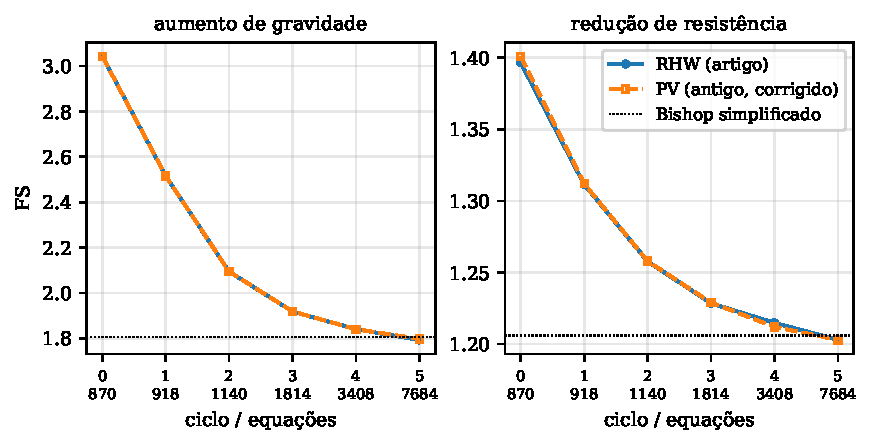
\includegraphics[width=0.92\textwidth]{fig_fs_refinement.pdf}
\caption{FS do talude seco em função do número de equações (refinamento da zona plástica).}\label{fig:fsdry}
\end{figure}

\begin{figure}[t]
\centering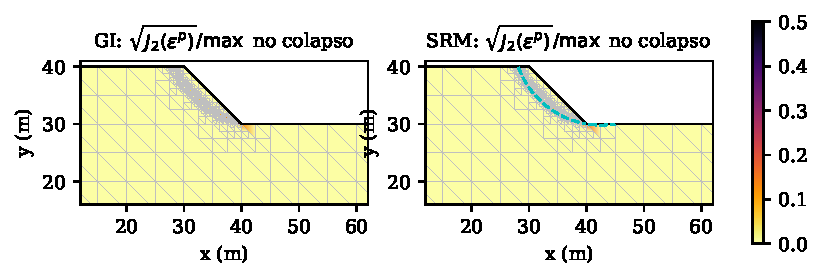
\includegraphics[width=0.98\textwidth]{fig_mechanism_dry.pdf}
\caption{Deformação plástica ($\sqrt{J_2(\eps^p)}$ normalizada) no colapso, malha do último ciclo:
aumento de gravidade (mecanismo raso) e SRM, com o círculo crítico de Bishop (tracejado).}\label{fig:mechdry}
\end{figure}

%=====================================================================================================
\section{Problema poroplástico: rebaixamento rápido (\code{SlopeDrawdown})}\label{sec:dd}

\subsection{Cenário}
Ceron, Cecílio, Linn e Maghous \cite{ceron2025} analisam por limite superior (mecanismos rotacionais
em espiral logarítmica) taludes submetidos a forças de percolação após o rebaixamento rápido total
($h_w=H$) do reservatório, com $c=\SI{10}{kPa}$, $\phi=30^\circ$ e $\gamma=\SI{20}{kN/m^3}$ --- os dados
deste talude. A análise hidráulica é ``parcialmente acoplada'': independe das deformações do
esqueleto, a linha freática permanece no topo e as forças de percolação $-\nabla p$ entram como forças
de volume, com resistência em tensões efetivas. Aqui o problema é resolvido com acoplamento completo
de Biot, cujo regime permanente é exatamente esse campo, e o FS é calculado pelo procedimento da
Seção~\ref{sec:slope} em cada instante.

\subsection{Formulação u--p}
O material \code{TPZMatPoroElastoPlasticUP} monta, a cada passo de Euler implícito,
\begin{align}
R_u &= F_{int}(U) - QP - f_b - \lambda f_t, &
R_p &= Q^T(U-U_n) + S(P-P_n) + \Delta t\,(HP-f_g),\\
K &= \begin{bmatrix} K_T & -Q\\ Q^T & S+\Delta t\,H\end{bmatrix}, &
K_T&=\int B^T\D B, \quad Q=\int\alpha B^T\mathbf m N_p,
\end{align}
$S=\int M^{-1}N_p^TN_p$, $H=\int k\nabla N_p^T\nabla N_p$, $f_g=\int k\nabla N_p^T\rho_w\mathbf g$,
$f_b=\int N_u^T\mathbf b$. O Mohr--Coulomb do artigo foi ligado ao material com uma instanciação explícita
e \code{LastProjectionFailed()} (a projeção fechada nunca falha). Como \code{TPZPlasticStepVoigt} é
formulado em deformação total, o estado inicial vem de um passo de gravidade (o $\sig'$ inicial da
memória é ignorado). Espaços: Taylor--Hood (u P2, p P1) em \code{TriGMesh(2)}; o driver
\code{TPZPoroElastoPlasticUPAnalysis} não renumera as equações, para que as de pressão fiquem depois
das de deslocamento e a LU sem pivotamento seja estável no passo não drenado ($S=0$, $\Delta t=0$).

\subsection{As duas funções pedidas}
O rascunho de \code{CreateCompMesh} vinha do exemplo triaxial de Cam-Clay; as correções foram:
\begin{itemize}
\item a malha de deslocamento não pode ser a malha elastoplástica (\code{CreateCMesh}): no espaço
  multifísico as malhas atômicas usam material nulo; \code{CreatePressureMesh} foi generalizada para
  \code{CreateAtomicMesh(gmesh, nstate, order, bcids)} ($n_{state}=2$ deslocamento P2, $1$ pressão P1);
\item as duas malhas atômicas precisam de \emph{todos} os ids de contorno usados na multifísica
  (a função forçante de um contorno é avaliada em \code{dataU.x});
\item \code{EPlaneStrain} (não \code{EThreeDimensional}); material com o Mohr--Coulomb
  (\code{mcc::TPoroMaterial} é Cam-Clay); nada de $p_c$, $v_0$ ou $\sig'_0$ na memória;
\item contornos do talude no lugar dos do triaxial (Tabela~\ref{tab:bc}); a pressão d'água e a carga
  d'água não podem ficar no mesmo id (um id tem uma só condição): elementos gêmeos $-13$ e $-16$
  (\code{TPZGeoElBC}) sobre $-3$ e $-6$;
\item o nível do reservatório $H=H_0-\lambda(H_0-H_1)$ é lido do fator de carga $\lambda$ do passo nas
  funções forçantes; a bissecção do driver interpola $\lambda$.
\end{itemize}

\begin{table}[h]
\centering\small
\begin{tabular}{@{}lll@{}}
\toprule
id & mecânico & hidráulico\\
\midrule
$-1$ base & fixo (\code{EDirichletU}) & impermeável\\
$-2$, $-5$ laterais & rolete $u_x=0$ (\code{EDirichletUDirectional}) & impermeável\\
$-3$ pé, $-6$ face & livre & $p=\gamma_w(H-y)^+$ (\code{EDirichletP})\\
$-4$ topo & livre & $p=0$ (linha freática no topo)\\
$-13$, $-16$ (gêmeos de $-3$, $-6$) & $\mathbf t=-\gamma_w(H-y)^+\mathbf n$ (\code{ENeumannUFixed}) & ---\\
\bottomrule
\end{tabular}
\caption{Condições de contorno da análise u--p.}\label{tab:bc}
\end{table}

CODE_LISTINGS

\subsection{Etapas}
\begin{enumerate}
\item reservatório no topo ($H_0=40$~m): gravidade aplicada em um passo drenado longo
  ($\Delta t=10^4H^2/c_v$, regime permanente hidrostático);
\item rebaixamento rápido até o pé ($H_1=30$~m): passo não drenado ($\Delta t=0$, $\lambda:0\to1$);
\item adensamento/percolação transiente: $T=c_vt/H^2=10^{-3}\dots10$ (4 passos por década) e um passo
  final até $T=10^4$ (regime permanente: campo de Ceron et al.).
\end{enumerate}
Dados: $E=\SI{20000}{kPa}$, $\nu=0{,}3$ (drenado; a resposta não drenada vem do acoplamento),
$c=\SI{10}{kPa}$, $\phi=\psi=30^\circ$, $\gamma_{sat}=\SI{20}{kN/m^3}$, $\gamma_w=\SI{10}{kN/m^3}$,
$\alpha=1$, $1/M=0$, $k=\SI{e-2}{m/dia}$. Então $M_{oed}=E(1-\nu)/[(1+\nu)(1-2\nu)]=\SI{26923}{kPa}$,
$c_v=kM_{oed}/\gamma_w=\SI{26.9}{m^2/dia}$ e $H^2/c_v=\SI{3.71}{dias}$ ($H=10$~m); os estados em $T$
não dependem de $k$.

\subsection{Estabilidade com forças de percolação}
Em cada estado, a poropressão $p(\mathbf x)$ (P1 por triângulo, valores nodais da análise u--p) é
congelada e o FS é calculado com \code{SlopeAnalysis.h} \emph{sem alteração} sobre a malha
elastoplástica de \code{SlopeMohrCoulomb}, trocando a força de volume por
\begin{equation}
\mathbf b = \lambda\,(\gamma_{sat}\,\mathbf g - \nabla p^+),\qquad p^+=\max(p,0),
\end{equation}
onde $\lambda$ é o fator de gravidade que \code{SlopeAnalysis} impõe pela força de volume do material.
Equivalência: com $\sig=\sig'-p\mathbf I$, a forma fraca em tensões totais, integrada por partes,
\begin{equation}
\int_\Omega B^T\sig'\,d\Omega = \int_\Omega(\gamma_{sat}\mathbf g-\nabla p)\cdot\mathbf v\,d\Omega
 + \int_\Gamma(\mathbf t+p\,\mathbf n)\cdot\mathbf v\,d\Gamma,
\end{equation}
e no contorno submerso $\mathbf t=-p_w\mathbf n$ com $p=p_w$: a tração efetiva é nula, e o problema
efetivo sem carga d'água é equivalente ao problema total. No aumento de gravidade $\lambda$ multiplica
$\gamma_{sat}$ \emph{e} $\nabla p$ (pesos do solo e da água), o que mantém a equivalência com $c/\lambda$
e com o fator de estabilidade $\Gamma=\lambda\gamma H/c$ de Ceron et al.; no SRM $\lambda=1$.
A sucção é desprezada ($p^+$).

%=====================================================================================================
\section{Resultados e verificação do rebaixamento}\label{sec:ddres}

\subsection{Poropressão}
A Figura~\ref{fig:pfields} mostra o campo de $p$ e a Figura~\ref{fig:pprof} perfis verticais.
\begin{itemize}
\item \textbf{Reservatório no topo}: $p=\gamma_w(40-y)$ (hidrostático) em todo o domínio, como deve ser.
\item \textbf{Logo após o rebaixamento} (não drenado): a retirada da carga d'água reduz a tensão
  total e, com fluido incompressível, a poropressão: sob o terreno baixo a queda é próxima da do
  carregamento unidimensional ($\Delta p\approx-\gamma_w\Delta H=-100$~kPa; PRESSURE_DROP), enquanto
  no maciço sob o topo $p$ quase não muda. A face e o pé ficam com $p=0$.
\item \textbf{Adensamento}: a água do maciço escoa para a face e o pé; $p$ cresce junto à face e ao
  pé e cai sob o topo, até o regime permanente de percolação com a linha freática no topo.
\end{itemize}

\begin{figure}[t]
\centering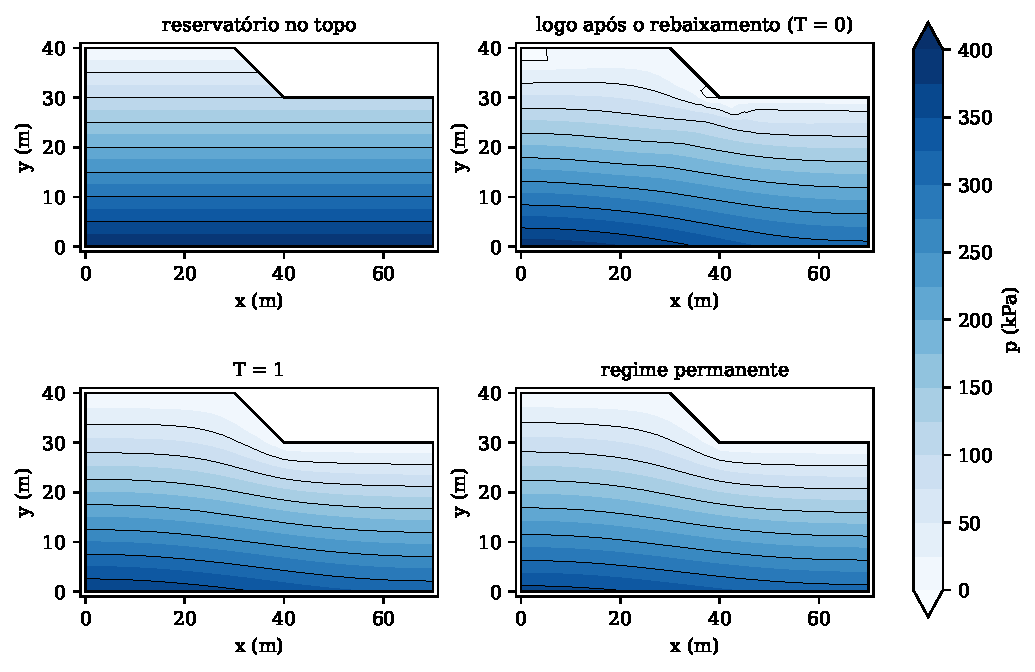
\includegraphics[width=0.98\textwidth]{fig_pressure_fields.pdf}
\caption{Poropressão da análise u--p em quatro instantes.}\label{fig:pfields}
\end{figure}

\begin{figure}[t]
\centering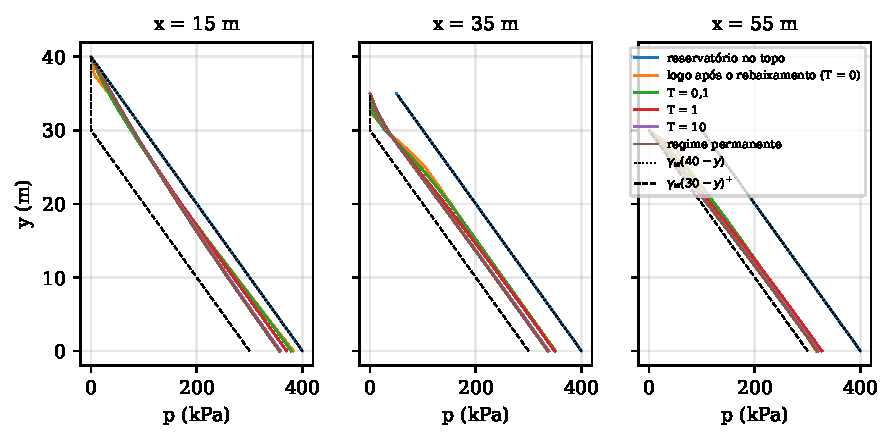
\includegraphics[width=0.98\textwidth]{fig_pressure_profiles.pdf}
\caption{Perfis verticais de poropressão sob o topo ($x=15$~m), sob a face ($x=35$~m) e sob o
reservatório ($x=55$~m).}\label{fig:pprof}
\end{figure}

\paragraph{Verificação independente da percolação.} LAPLACE_CHECK

\subsection{Fator de segurança}
FS_DISCUSSION

\begin{figure}[t]
\centering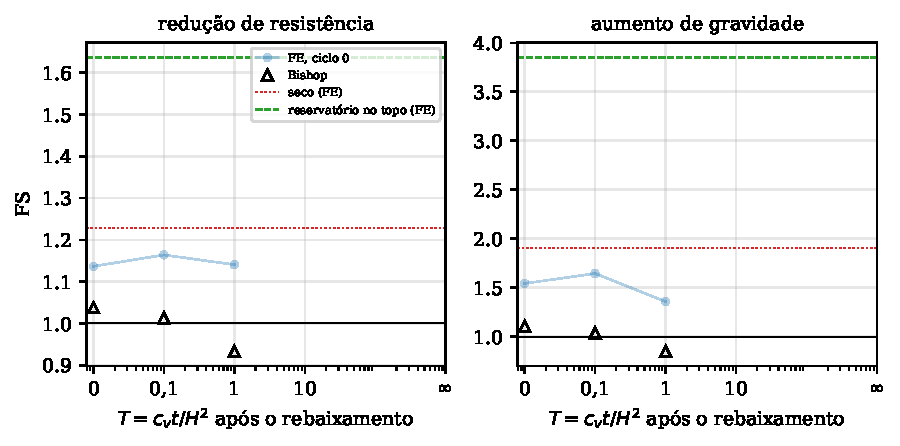
\includegraphics[width=0.98\textwidth]{fig_fs_time.pdf}
\caption{FS após o rebaixamento em função de $T=c_vt/H^2$ (ciclos de refinamento em tons crescentes),
Bishop com o mesmo campo $p^+$ ($\triangle$) e os estados seco e com o reservatório no topo.}\label{fig:fstime}
\end{figure}

\begin{figure}[t]
\centering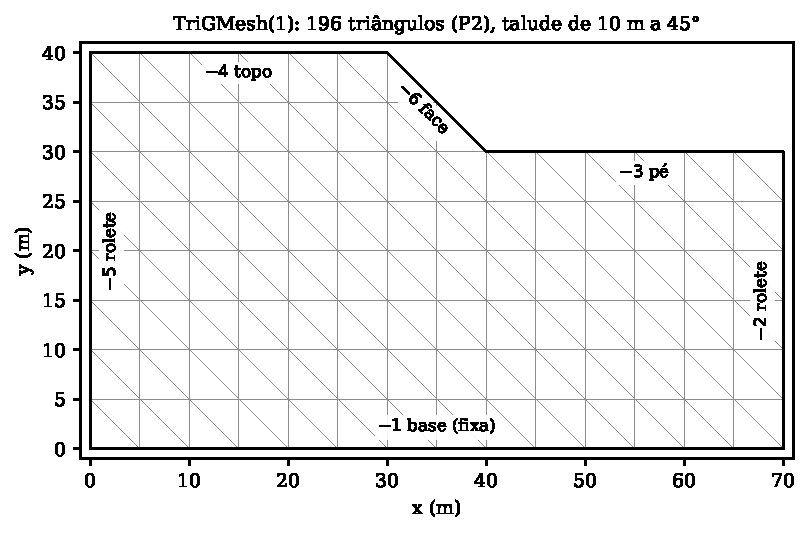
\includegraphics[width=0.98\textwidth]{fig_mechanism_drawdown.pdf}
\caption{Mecanismo de ruptura do SRM logo após o rebaixamento e em regime permanente, com o círculo
crítico de Bishop.}\label{fig:mechdd}
\end{figure}

\subsection{Convergência da análise u--p}
Todos os passos convergem sem bissecção. No passo drenado de gravidade
$\|R\|/\|F\|$: $10{,}1\to8\cdot10^{-3}\to3{,}7\cdot10^{-3}\to6\cdot10^{-4}\to5{,}8\cdot10^{-6}\to1{,}3\cdot10^{-9}$;
nos passos de adensamento são 6 a 8 avaliações, com a fase final quadrática. As primeiras iterações
são mais lentas porque pontos mudam entre elástico e plástico e porque o resíduo normalizado mistura
as linhas de pressão (escaladas por $\Delta t$) com as de deslocamento --- comportamento do driver,
igual ao dos exemplos de Cam-Clay.

%=====================================================================================================
\section{Limitações}
\begin{itemize}
\item Modelo saturado: a face acima d'água é tratada com $p=0$ e a sucção é desprezada no FS; o
  rebaixamento da linha freática dentro do maciço (fluxo não confinado) não é modelado --- coerente
  com a hipótese de rebaixamento rápido de Ceron et al.
\item Mohr--Coulomb associativo: no passo não drenado a dilatância plástica geraria sucção; o ganho
  de resistência correspondente é desprezado no FS (análise drenada com $p^+$ congelado).
\item O FS por gravidade só converge com o refinamento da zona plástica (mecanismo raso); os valores
  da malha inicial são apenas indicativos.
\item Pendências da biblioteca na Seção~\ref{sec:bugs}.
\end{itemize}

%=====================================================================================================
\section{Como reproduzir}
\begin{lstlisting}[language=bash]
cmake -DBUILD_PLASTICITY_MATERIALS=ON -DBUILD_PROJECTS=ON <neopz>
ninja SlopeMohrCoulomb SlopeDrawdown
SLOPE_VERBOSE=1 ./SlopeMohrCoulomb nref=4 > out.txt   # talude seco (+ "check": teste de Taylor)
./SlopeDrawdown nref=3 > out.txt                      # rebaixamento rapido
python docs/slope_mohr_coulomb/scripts/make_figures.py <seco> <rebaixamento> <taylor.csv> <laplace> figs
\end{lstlisting}
Os scripts de verificação independente (Bishop com poropressão, solução P1 da percolação, teste de
Taylor) estão em \code{docs/slope_mohr_coulomb/scripts}.

\begin{thebibliography}{9}
\bibitem{lira2026} D.~Lira Cecílio. Return mapping for Mohr--Coulomb plasticity in rotated
  Haigh--Westergaard space with consistent tangent operator. \emph{J.\ Eng.\ Math.} 157:10, 2026.
\bibitem{ceron2025} M.~V.~Ceron, D.~Lira Cecílio, R.~V.~Linn, S.~Maghous. Stability analysis of slope
  subjected to seepage forces considering spatial variability of soil properties. \emph{Int.\ J.\ Numer.\
  Anal.\ Methods Geomech.} 49(11):2459--2491, 2025. doi:10.1002/nag.3993.
\bibitem{souza} E.~A.~de Souza Neto, D.~Perić, D.~R.~J.~Owen. \emph{Computational Methods for
  Plasticity}. Wiley, 2008.
\bibitem{gl99} D.~V.~Griffiths, P.~A.~Lane. Slope stability analysis by finite elements.
  \emph{Géotechnique} 49(3):387--403, 1999.
\bibitem{lg00} P.~A.~Lane, D.~V.~Griffiths. Assessment of stability of slopes under drawdown
  conditions. \emph{J.\ Geotech.\ Geoenviron.\ Eng.} 126(5):443--450, 2000.
\end{thebibliography}
\end{document}
